\documentclass{article}
\usepackage{geometry,tikz}
\usetikzlibrary{arrows,decorations.markings}
\geometry{paperwidth=12.5cm,paperheight=6.8cm,left=2pt,right=2pt,top=2pt,bottom=2pt}
\pagestyle{empty}
\setlength{\parindent}{0pt}
\tikzset{%
object/.style={draw,font=\tt},
create/.style={draw,-o},
filled/.style={draw,-*},
contains/.style={draw,-(,dashed},
createfill/.style={draw,decoration={markings,
                                    mark= at position -6.5pt with {
                                                      \fill[white,draw=black](0,0)   circle(2.5pt);
                                                      \fill[black]           (4.5pt,0) circle(2.5pt);
                                                                }
                                   },
                                   postaction={decorate}}
}
\begin{document}
\centering
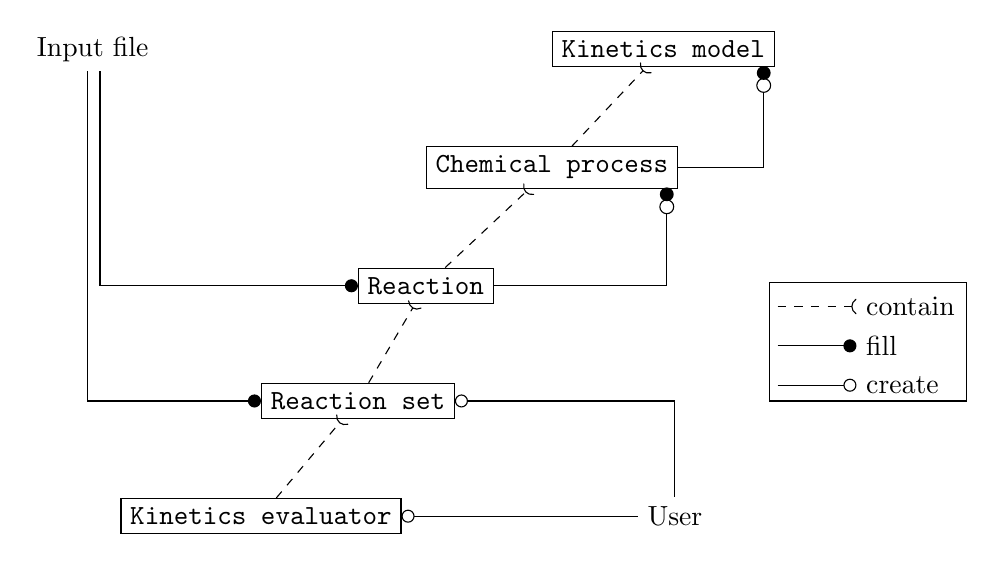
\begin{tikzpicture}
\node[object]             (kinmol)   at (0,0)                 {Kinetics model};
\node[object,below = 1cm] (chemproc) at (kinmol.south west)   {Chemical process};
\node[object,below = 1cm] (reac)     at (chemproc.south west) {Reaction};
\node[object,below = 1cm] (reacset)  at (reac.south west)     {Reaction set};
\node[object,below = 1cm] (kineval)  at (reacset.south west)  {Kinetics evaluator};
\foreach \m/\c in {kineval/reacset,
                   reacset/reac,
                   reac/chemproc,
                   chemproc/kinmol}
{
  \draw[contains] (\m) -- (\c);
}
\node[left=5cm]  (file) at (kinmol.west)   {Input file};
\node[right=3cm] (user) at (kineval.east) {User};

\foreach \o/\xs in {reac/10,reacset/-10}
  \draw[filled] ([xshift=\xs mm]file) |- (\o);

\foreach \f/\o in {reac/chemproc,chemproc/kinmol}
  \draw[createfill] (\f.east) -| ([xshift=-4pt]\o.south east);

\draw[create] (user) -- (kineval);
\draw[create] (user) |- (reacset);

\draw ([xshift=4cm]reacset.east)coordinate (leg) rectangle +(2.5,1.5);

\draw[create]   ([yshift=2mm,xshift=1mm]leg) -- ++(1,0)node[right]{create};
\draw[filled]   ([yshift=7mm,xshift=1mm]leg) -- ++(1,0)node[right]{fill};
\draw[contains] ([yshift=1.2cm,xshift=1mm]leg) -- ++(1,0)node[right]{contain};
\end{tikzpicture}
\end{document}
